
% \documentclass{beamer}
% % početak: može, ali ne mora
% \usetheme{metropolis} % {default} {Goettingen} {Copenhagen}
% \setbeamercovered{transparent} % ovo je važno za dinamiku
% \usecolortheme{default} % {seahorse}{rose}{wolverine}{infolines}
% % kraj: može, ali ne mora
% \usepackage[utf8]{inputenc}
% \usepackage[T1, T2A]{fontenc}
% \usepackage[serbianc]{babel}
% \usepackage{datetime}
% \title[prezentacija]{\huge prezentacija}
% \date{\today}
% \begin{document}
% \begin{frame}
% \titlepage
% \end{frame}
% \end{document}

\documentclass{beamer}
\usetheme{metropolis}           % Use metropolis theme {metropolis}

\setbeamercovered{transparent}

\usepackage[utf8]{inputenc}
\usepackage[T1, T2A]{fontenc}
\usepackage[serbianc]{babel}
\usepackage{datetime}

\usepackage[labelformat=empty]{caption}
%%%%%%%%%%%%%%%%%%%%%%%%%%%
\usepackage{amsmath}
\usepackage{mathtools}
\DeclarePairedDelimiter\ceil{\lceil}{\rceil}
\DeclarePairedDelimiter\floor{\lfloor}{\rfloor}
%%%%%%%%%%%%%%%%%%%%%%%%%%%
\usepackage{float}
\usepackage{minted}
\usepackage{verbatim}
\usepackage{cite}

\bibliographystyle{ieeetr}
%\setlength{\bibsep}{0.0pt}

\hypersetup{
    colorlinks=true,
    linkcolor=black,
    citecolor=black,
    filecolor=magenta,
    urlcolor=cyan,
}
\makeatletter
\g@addto@macro\UrlBreaks{\do\-}
%\g@addto@macro{\UrlBreaks}{\UrlOrds}
\makeatother


% \AtBeginSection[]
% {
%   \begin{frame}
%     \frametitle{Садржај}
%     \tableofcontents[currentsection]
%   \end{frame}
% }

\title{\alert{Мастер рад}\\
Хардверска дигитална мрежа за сортирање}
%\date{\today}
\date{28.\ септембар 2023.}
\author{\alert{Студент: Алекса Величковић 2020/3358} \\
Ментор: доц.\ др Живојин Шуштран}
\institute{Универзитет у Београду \\
Електротехнички факултет}

% logo of my university
\titlegraphic{%
  \begin{picture}(0,0)
    \put(305,-165){\makebox(0,0)[rt]{
\includegraphics[scale=0.15]{slike/etf}}}
  \end{picture}}

\begin{document}
\maketitle

%\section{Увод}

\begin{frame}
\frametitle{Рекурзивна имплементација битоник сортера у Чизелу}

 \begin{itemize}
  \item Описана је рекурзивна имплементација хардверске дигиталне мреже за сортирање битоник сортер
  \item Имплементација је урађена коришћењем језика за опис хардвера Чизел, базиран на програмском језику Скала
  \begin{itemize}
   \item Oмогућава једноставније дефинисање хардвера од других језика и прегледнији програмски код
   % за моделовање хардвера
  \end{itemize}
  \item Приказана су постојећа решења, са којим се врше поређења
 \end{itemize}
\hspace{1cm}
 \begin{figure}[H]
   \centering
%       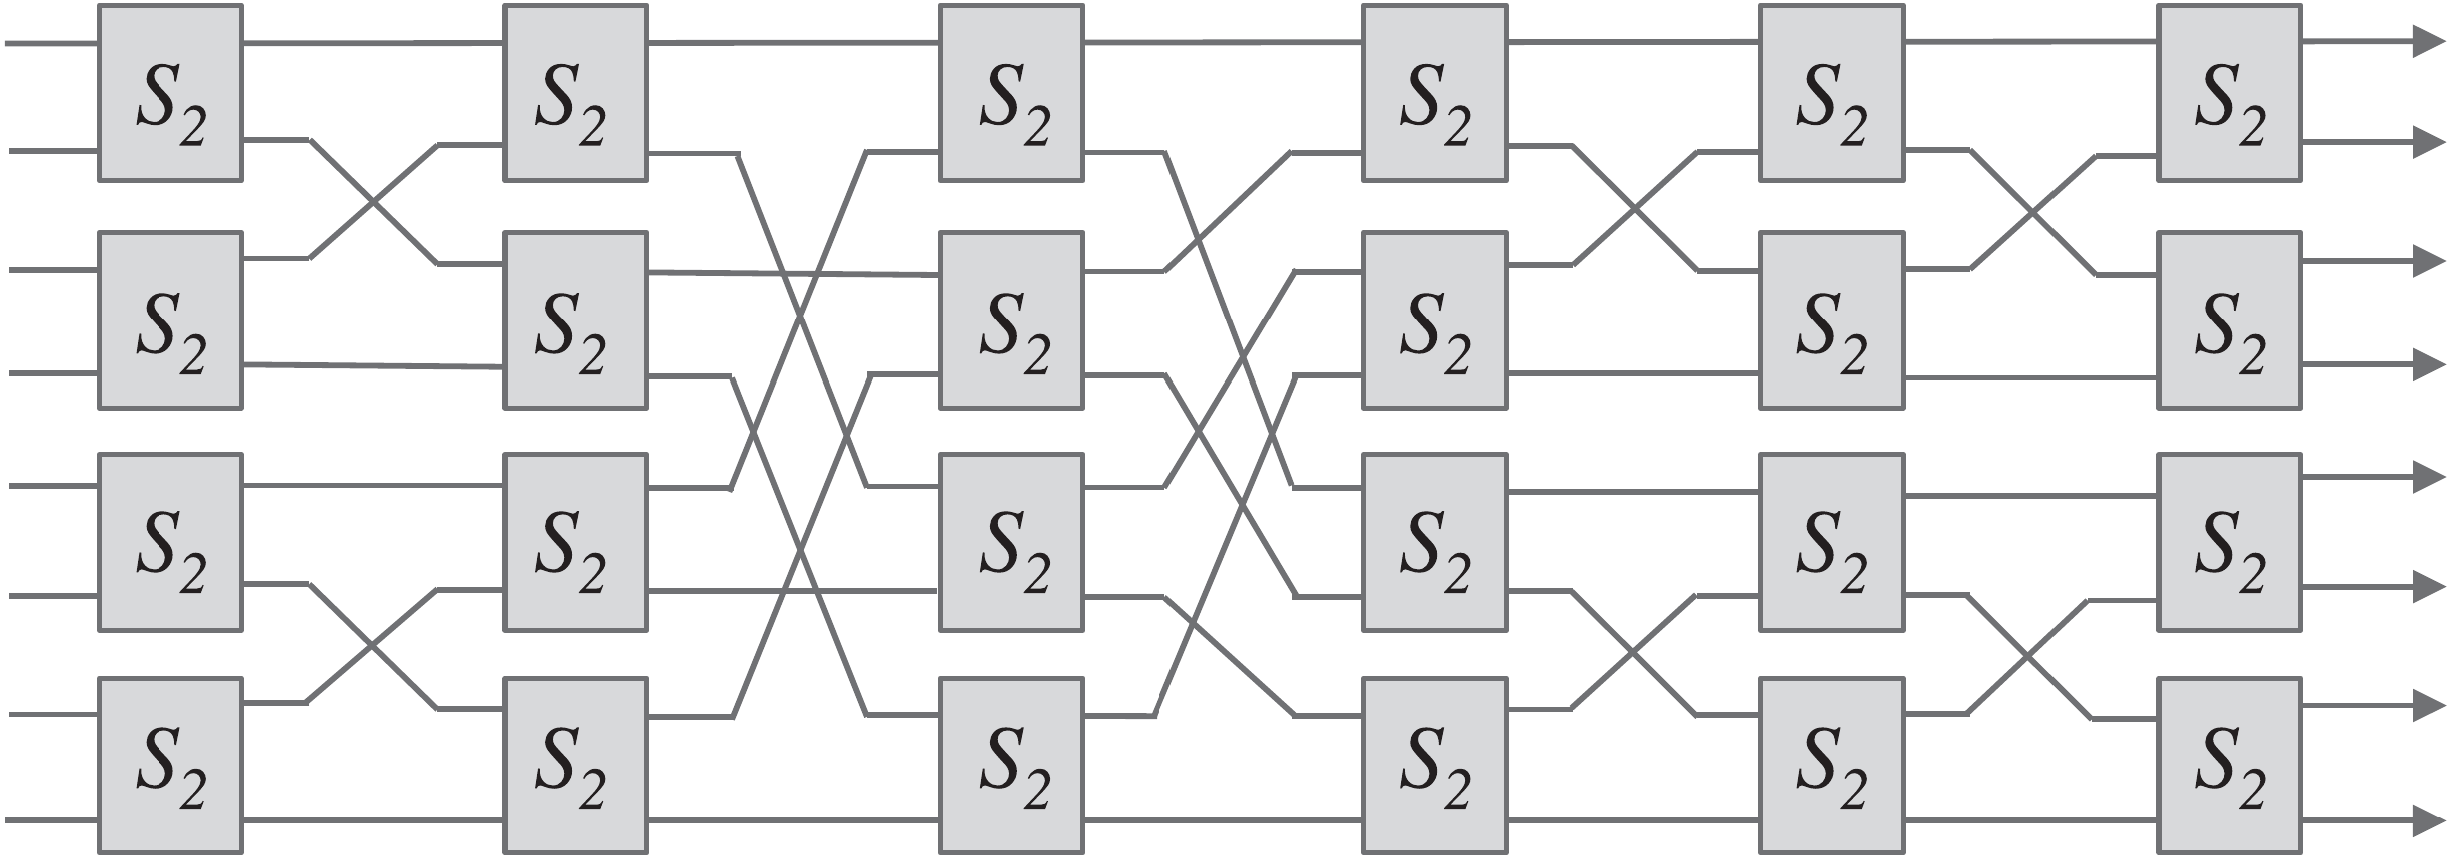
\includegraphics[scale=0.08]{slike/mreza} \hspace{0.4cm}
       
\includegraphics[scale=0.5]{slike/chisel_logo.pdf}
 \end{figure}

\end{frame}

%%%%%%%%%%%%%%%%%%%%%%%%%%%%%%%%%%%%%%%%%%%%%%%%%%%%%%
%\section{Коришћени алати}
%%%%%%%%%%%%%%%%%%%%
%\subsection{Скала}
\begin{frame}
\frametitle{Скала}

 \begin{itemize}
  \item Скала (енг. \textit{Scala}) је програмски језик који подржава и објектно-оријентисано и функционално програмирање
  \item Дизајниран је да буде концизан и да надомести недостатке које има програмски језик Јава (енг. \textit{Java})
  \item Постоjе многи софтверски алати коjи су написани у Скали или су надограђени на овом програмском jезику
%  \item Функција \alert{extract\_card()} издваја карту са прослеђене слике
%  \begin{itemize}
%   \item Провера замућења слике; смањење шума; издвајање ивица (прелаза)
%   са слике и налажење контура (спаја све тачке дуж границе,
%   исте боје и интензитета)
%   \item Требало би да је највећа контура карта;
%   проверава се да ли је приближно правоугаоног облика
%   \item Простор унутар контуре се претвара у правоугаоник
%   димензија карте (шаблона)
  \end{itemize}

 \begin{figure}[H]
   \centering
       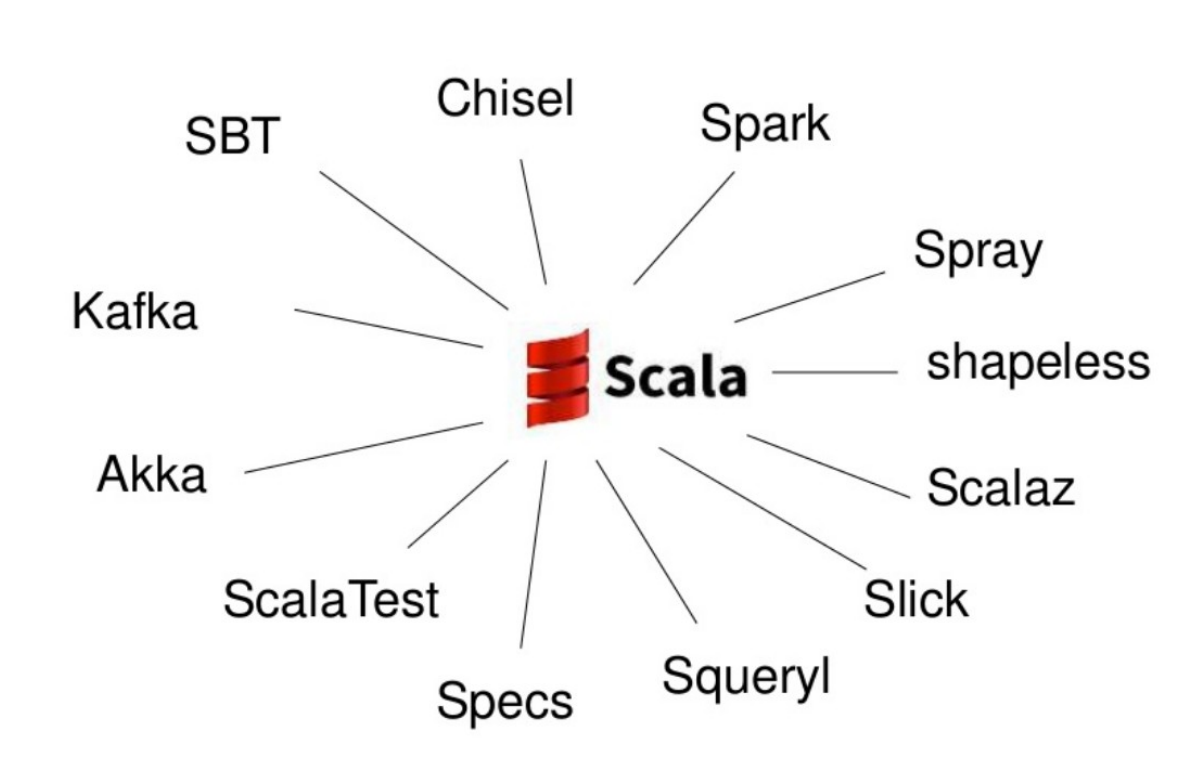
\includegraphics[scale=0.2]{slike/scalaDer.png}
  \end{figure}
\end{frame}
%%%%%%%%%%%%%%%%%%%%
%\subsection{Чизел}
\begin{frame}[fragile]
\frametitle{Чизел}
 \begin{itemize}
  \item \alert{Чизел} је језик за опис хардвера заснован на програмском језику Скала %(енг. \textit{Chisel - Constructing Hardware in a Scala Embedded Language})
  \begin{itemize}
   \item \textit{Chisel - Constructing Hardware in a Scala Embedded Language}
   \item Наслеђује аспекте ООП и ФП Скале
   \item Битно је разликовати који типови, оператори, условни изрази припадају Скали, а који Чизелу
   \item Чизел програмски код може бити претворен у Верилог за синтезу и симулацију
   \item Захтева много мање кода од Верилога
  \end{itemize}
 \end{itemize}
 \begin{minted}[fontsize=\footnotesize]{scala}
    class RegisterModule extends Module {
      val io = IO(new Bundle {
        val in  = Input(UInt(12.W))
        val out = Output(UInt(12.W))
      })
      val register = Reg(UInt(12.W))
      register := io.in + 1.U
      io.out := register }
\end{minted}
\end{frame}

%%%%%%%%%%%%%%%%%%%%
% \subsection{Радна окружења и алати}
% \begin{frame}
% \frametitle{Радна окружења и алати}
% \begin{itemize}
%  \item Јупитер свеска и Докер
%  \item Intellij и SBT
%  \item Quartus Prime Lite
% \end{itemize}
% \begin{figure}[H]
%   \centering
%       \includegraphics[scale=0.18]{slike/dveKarte.jpg} \hspace{1.2cm}
%       \includegraphics[scale=0.18]{slike/triKarte.jpg}
%  \end{figure}
% \end{frame}

%%%%%%%%%%%%%%%%%%%%%%%%%%%%%%%%%%%%%%%%%%%%%%%%%%%%%%
%\section{Мреже за сортирање}

\begin{frame}
\frametitle{Мреже за сортирање}

 \begin{itemize}
  \item \alert{Мреже за сортирање} паралелно обрађуjу листу n улазних елемената кроз више нивоа тако да jе на последњем нивоу улазна листа сортирана
  %\item Током сваког нивоа паралелно се изводе поређења и пермутациjе
  \item Број улазних вредности је степен броја два: $n = 2^t$
  \item Броj нивоа и броj поређења по нивоу одређуjу цену мреже
  \begin{itemize}
   \item Битоник сортер на слици има $\log_{2}(n)(\log_{2}(n)+1)/2$ нивоа са $n/2$ паралелних $S_2$ операција, укупно $\mathcal{O}(n\log^2 n)$ оп.
  \end{itemize}
 \end{itemize}

 \begin{figure}[H]
   \centering
       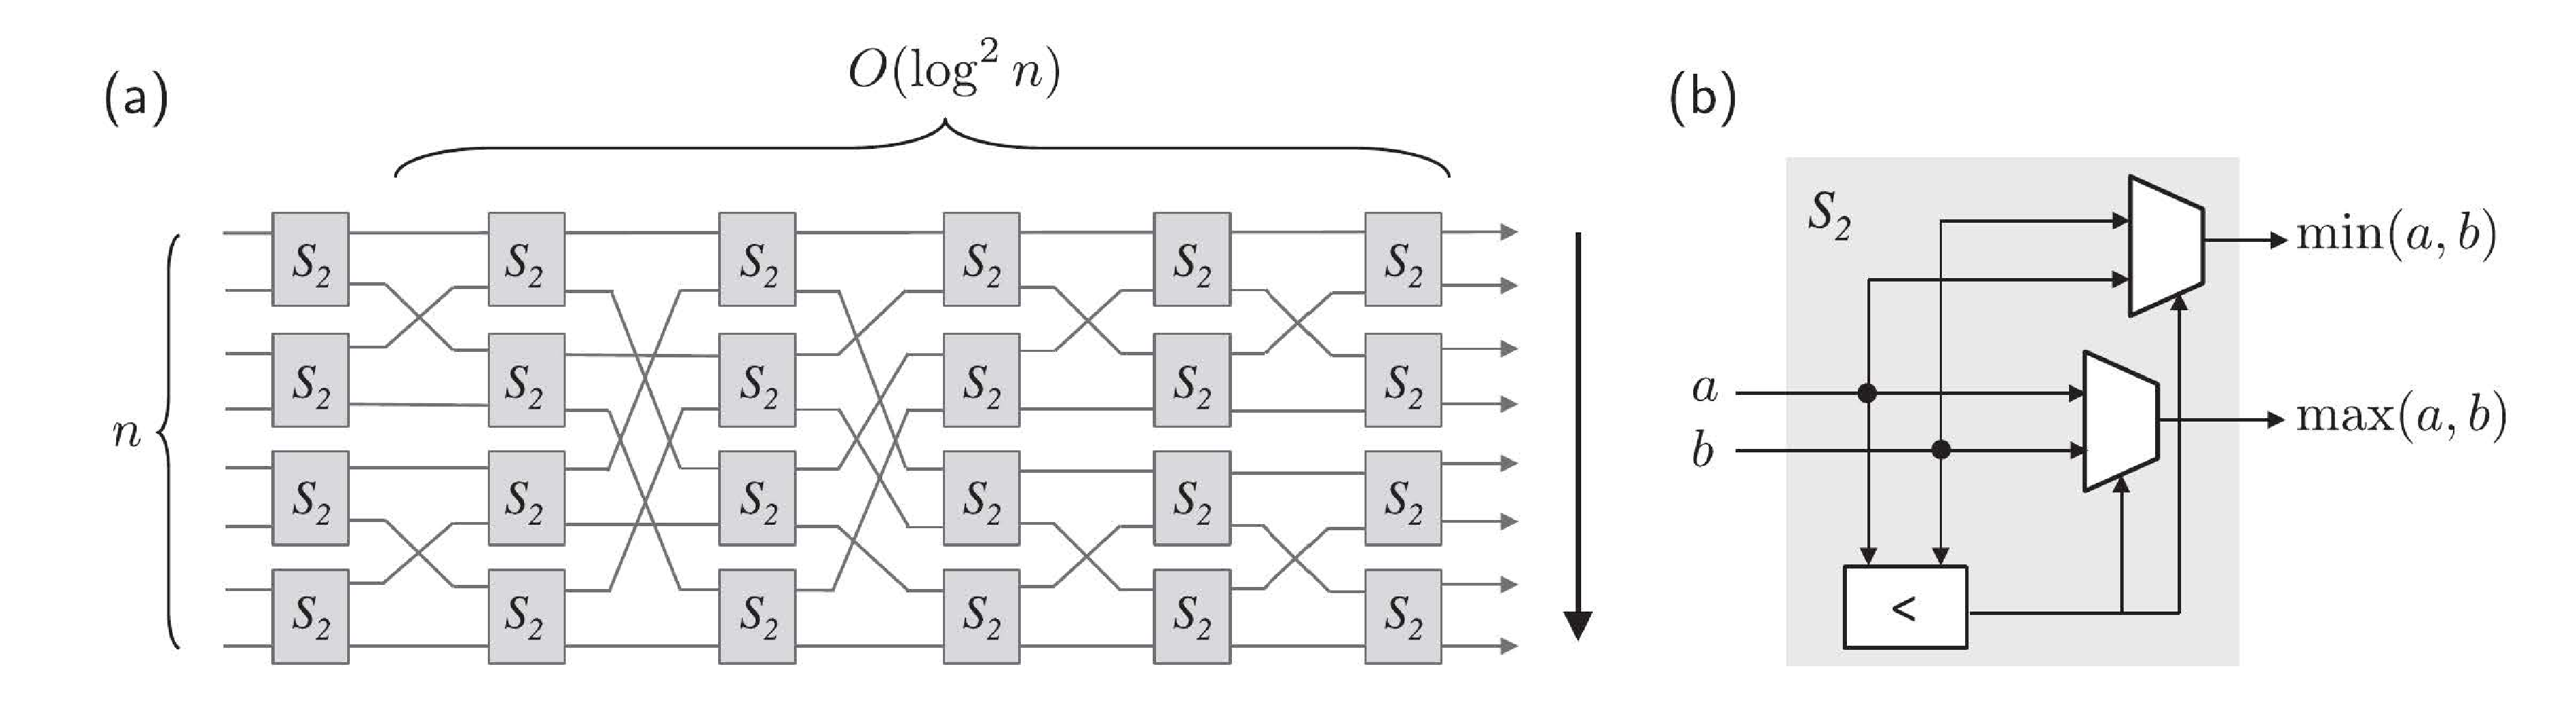
\includegraphics[scale=0.15]{slike/bitonicStages.pdf}
 \end{figure}

\end{frame}

%%%%%%%%%%%%%%%%%%%%
%\subsection{Битоник сортер}
\begin{frame}
\frametitle{Битоник сортер}
 \begin{itemize}
  \item \textit{Bitonic mergesort} aлгоритам је објавио Кенет Едвард Бечер 1968.\ године. Tакође је развио и \textit{пар-непар} (\textit{odd-even}) мреже за сортирање
  \begin{itemize}
   \item Најпопуларнија решења, због једноставности, и близине оптималној цени и перформансама
  \end{itemize}
  \item \alert{Битоник низ} се састоји из два монотона низа, растућег и опадајућег
  \item Унутар црвених правоугаоника се пореде елементи из горње половине са одговарајућим из доње. Излаз из плавог је растући, из зеленог опадајући
 \end{itemize}
\begin{figure}[H]
  \centering
      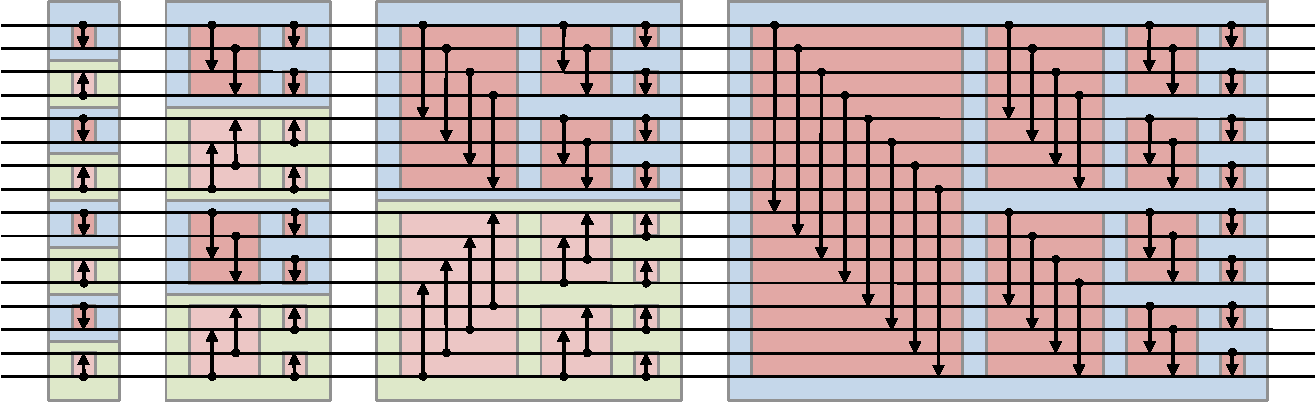
\includegraphics[scale=0.35]{slike/BitonicSort1.pdf}
 \end{figure}
\end{frame}

%%%%%%%%%%%%%%%%%%%%%%%%%%%%%%%%%%%%%%%%%%%%%%%%%%%%%%
%\section{Постојећа решења}

%%%%%%%%%%%%%%%%%%%%
%\subsection{Итеративна имплементациjа битоник сортера у Чизелу}
\begin{frame}[fragile]
\frametitle{Итеративна имплементациjа битоник сортера у Чизелу}
 \begin{itemize}
  \item Програмски код искоришћен за имплементацију рекурзивног решења
  \item Класа \verb+Swapper+ дефинише хардверски модул за замену два улазна елемента на основу функције поређења.
  \item \verb+insertSorter+ jе помоћна функциjа коjа врши замену елемената задатим са \verb+lo+ и \verb+hi+
  \item Главна логика се извршава у петљи, где \verb+i+ представља битну позицију која се разматра, \verb+j+ варира од \verb+i+ до \verb+0+, и \verb+k0+ и \verb+k1+ итерирају кроз елементе који треба да се пореде
  \item Генерисан је Верилог код и извршена синтеза у Quartus-у
 \end{itemize}
% \begin{minted}[fontsize=\footnotesize]{scala}
% (for {
%     i <- 0 until log2Up(a.length)
%     j <- i to 0 by -1
%     k0 <- a.indices by (2 << j)
%     k1 <- 0 until 1 << j
%   } yield {
%     val lo = k0 + k1
%     val hi = lo + (1 << j)
%     if ((lo >> (i + 1)) % 2 == 0) (lo, hi) else (hi, lo)
%   }).foldLeft(a) { case (s, (l, h)) => insertSorter(s, l, h) }
% \end{minted}

\begin{figure}[H]
  \centering
      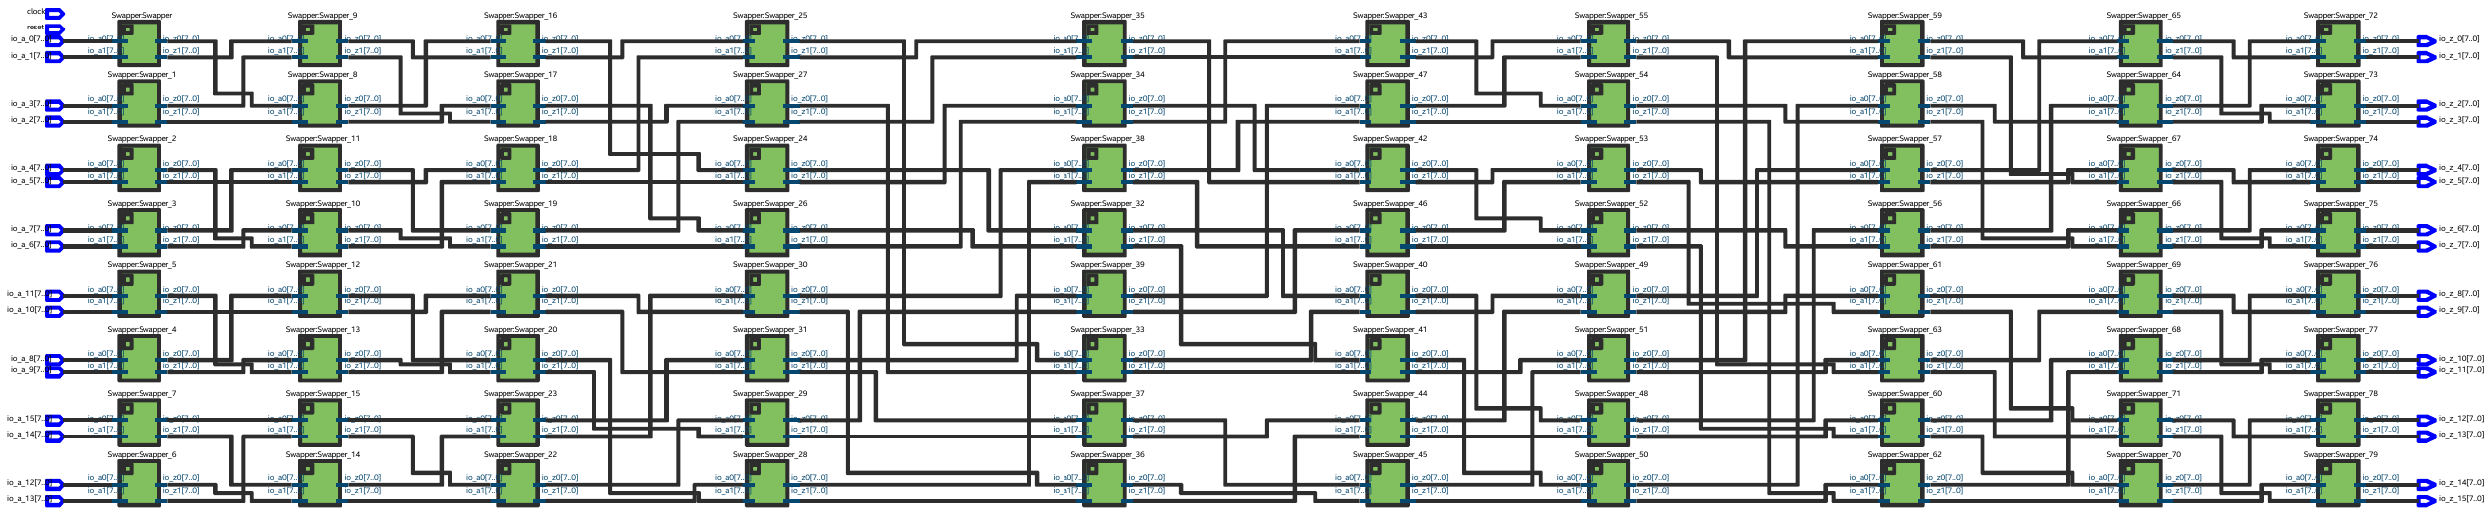
\includegraphics[scale=0.15]{slike/RTL_Iter_16_8.png}
 \end{figure}
\end{frame}

%%%%%%%%%%%%%%%%%%%%
%\subsection{Рекурзивна имплементација у Пајтону}
\begin{frame}[fragile]
\frametitle{Рекурзивна имплементација у Пајтону}
 \begin{itemize}
 %\item \verb+compAndSwap(a, i, j, dire)+ функција служи за упоређивање и замену два елемента у низу
  \item \verb+bitonicMerge(a, low, cnt, dire)+ функција \alert{рекурзивно сортира битоник низ} у растућем или опадајућем редоследу, у зависности од вредности параметра \verb+dire+. Низ се сортира почевши од позиције \verb+low+, а параметар \verb+cnt+ представља број елемената који се сортирају.
  \item \verb+bitonicSort(a, low, cnt, dire)+ функција прво \alert{производи битоник низ} рекурзивним сортирањем његовe две половине у супротним редоследима, а затим позива функцију \verb+bitonicMerge+ да их уједини у исти редослед
 \end{itemize}
%  \begin{minted}[fontsize=\footnotesize]{python}
%     def bitonicSort(a, low, cnt,dire):
%       if cnt > 1:
%         k = cnt//2
%         bitonicSort(a, low, k, 1)
%         bitonicSort(a, low+k, k, 0)
%         bitonicMerge(a, low, cnt, dire)
%  \end{minted}
  \begin{minted}[fontsize=\footnotesize]{python}
    def bitonicMerge(a, low, cnt, dire):
      if cnt > 1:
        k = cnt//2
        for i in range(low , low+k):
            compAndSwap(a, i, i+k, dire)
        bitonicMerge(a, low, k, dire)
        bitonicMerge(a, low+k, k, dire)
  \end{minted}

\end{frame}

%%%%%%%%%%%%%%%%%%%%
%\subsection{Имплементација битоник сортера у Верилогу}
\begin{frame}[fragile]
\frametitle{Имплементација битоник сортера у Верилогу}
 \begin{itemize}
 %\item Пројекат се састоји од 4 модула \verb+bitonic_node+, \verb+bitonic_comp+, \verb+bitonic_block+ и \verb+bitonic_sort+, где је \verb+bitonic_sort+ на највишем нивоу:
  \item \verb+bitonic_comp+ - компаратор и логика замене
  \item \verb+bitonic_node+ - основна jединица битоник мреже
  \begin{itemize}
   \item Производи сортиране излазе, састоји се од \verb+bitonic_comp+
  \end{itemize}
  \item \verb+bitonic_block+ представља степен (ниво) у битоник мрежи за сортирање
  \begin{itemize}
   \item Унутар овог модула има више инстанци модула \verb+bitonic_node+ које чине битоник мрежу овог степена
  \end{itemize}
  \item \verb+bitonic_sort+ модул je на највишем нивоу и представља потпуну битоник мрежу за сортирање.
  \begin{itemize}
    \item Управља сортирањем података делећи га на степене и блокове користећи модуле \verb+bitonic_block+ и \verb+bitonic_node+.
  \end{itemize}
 \end{itemize}

 \begin{figure}[H]
  \centering
      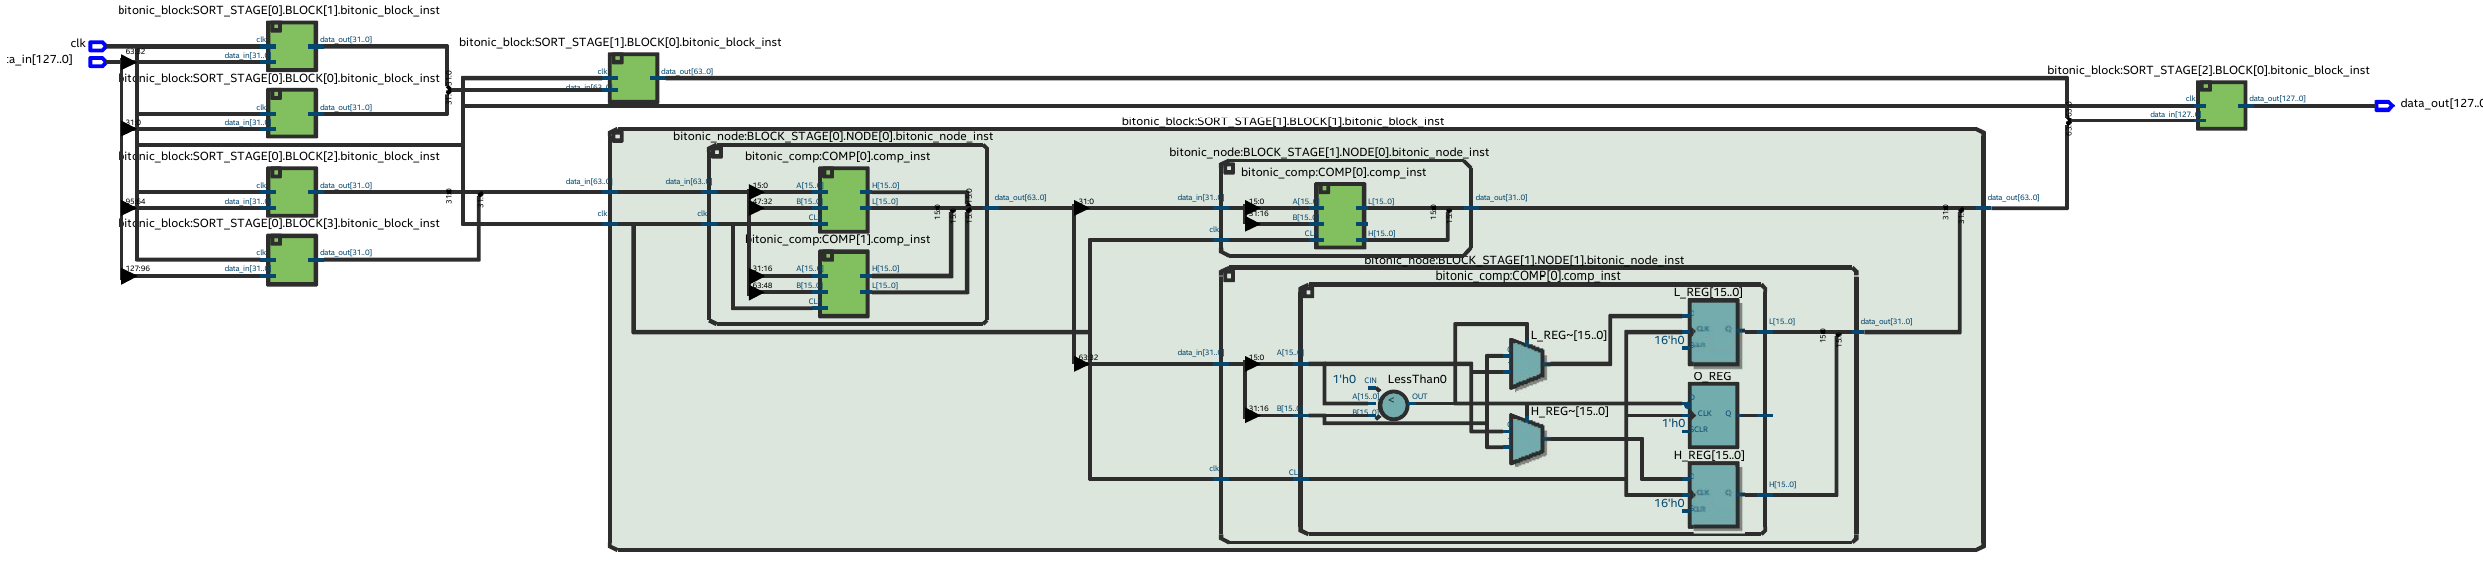
\includegraphics[scale=0.15]{slike/rtl_verilog}
 \end{figure}
\end{frame}


%%%%%%%%%%%%%%%%%%%%
%\subsection{Рекурзивна имплементација битоник сортера у Чизелу}
\begin{frame}[fragile]
\frametitle{Рекурзивна имплементација битоник сортера у Чизелу}
 \begin{itemize}
 \item Као основа за израду ове имплементације су искоришћене итеративна у Чизелу и рекурзивна у Пајтону
 \item Објекат \verb+BitonicSorter+ дефинише функције: \verb+bitonicMerge()+, \verb+bitonicSort()+ и \verb+sort()+.
 \end{itemize}

    \begin{minted}[fontsize=\footnotesize]{scala}
    def swapIfNecessary(...): IndexedSeq[Option[T]] = {
      val j = i + length / 2
      val si = arr(i).getOrElse(0.U.asTypeOf(arr(i).get))
      val sj = arr(j).getOrElse(0.U.asTypeOf(arr(j).get))
      val m = Module(new Passthrough(si.cloneType))
      val swapNeeded = lt(sj, si) === ascending
      when(swapNeeded) {
        m.io.a0 := sj
        m.io.a1 := si
      }.otherwise {
        m.io.a0 := si
        m.io.a1 := sj }
      seq.updated(i, Some(m.io.z0)).updated(j, Some(m.io.z1)) }
  \end{minted}
\end{frame}

\begin{frame}[fragile]
\frametitle{Рекурзивна имплементација битоник сортера у Чизелу}
  \begin{itemize}
  \item Потребно је генерисати нову листу са замењеним (свапованим) елементима у одговарајућем редоследу, у \verb+bitonicMerge()+ функцији, искорићена је \verb+foldLeft()+ функција, која извршава функцију \verb+swapIfNecessary()+
    \begin{minted}[fontsize=\footnotesize]{scala}
  val indices = 0 until half
  val swappedSeq = indices.foldLeft(arr) { (seq, i) =>
    swapIfNecessary(seq, i, ascending, lt) }
  \end{minted}
  \item Тестирање је извршено за низове дужине 1, 2, 4, 8, 16 који се састоје од насумичних бројева ширине 8, 16, 32, 64 бита
  \item Позивом \verb+getVerilog(new BitonicSorterModule(...)+ је добијен Верилог код и синтеза је извршена у Quartus-y
  \end{itemize}
  \begin{figure}[H]
  \centering
      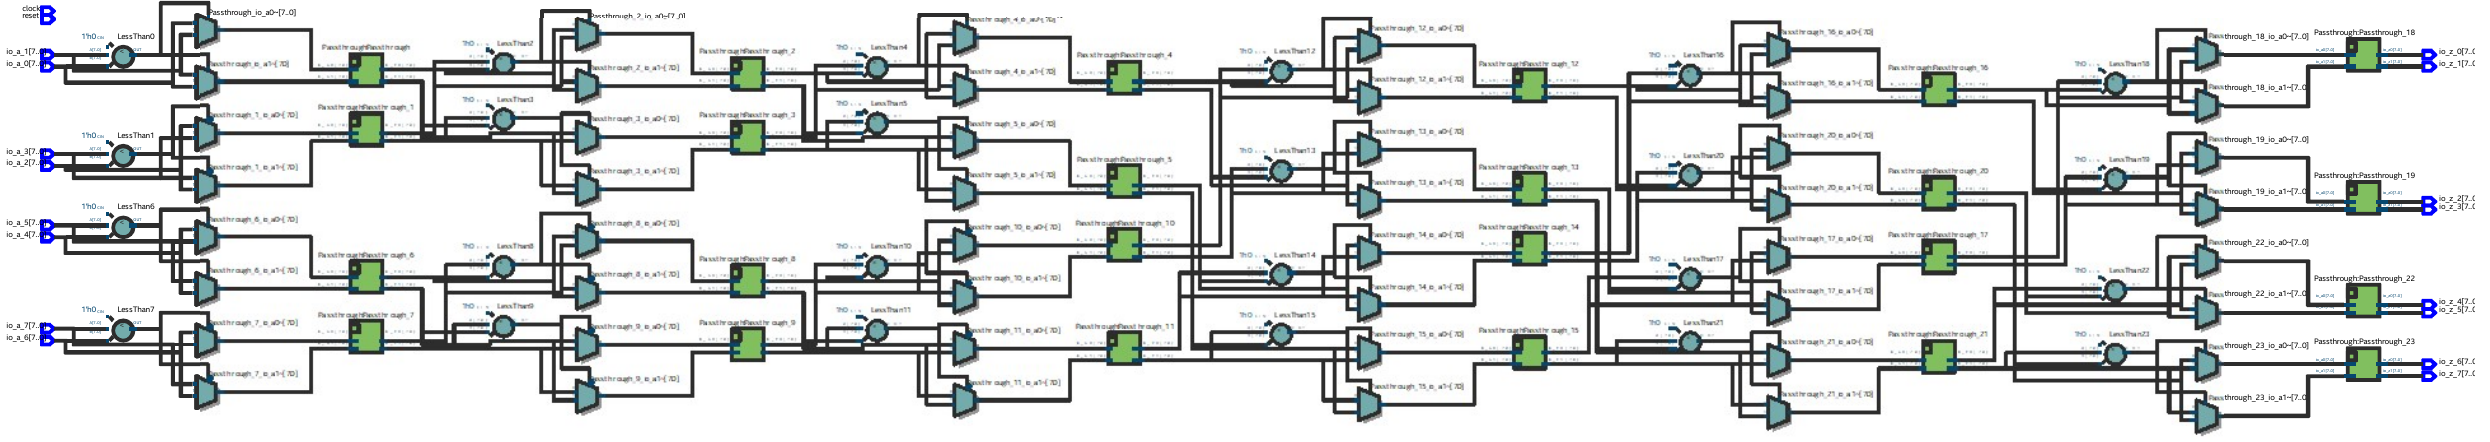
\includegraphics[scale=0.15]{slike/RTL_Rec_8_8.png}
 \end{figure}
\end{frame}

%%%%%%%%%%%%%%%%%%%%
%\subsection{Поређење са претходним имплементацијама}
\begin{frame}%[fragile]
\frametitle{Поређење са претходним имплементацијама}
 \begin{itemize}
 \item Следећи графици приказују број Look-up табела потребних за синтезу приказаних имплементација на FPGA уређају Cyclone V 5CGXFC9E7F35C8 када је број елемената за сортирање 8 и 16
 \item Итеративна и рекурзивна имплементациjа у Чизелу заузимају готово исти простор на чипу
 \end{itemize}
   \begin{figure}[H]
  \centering
      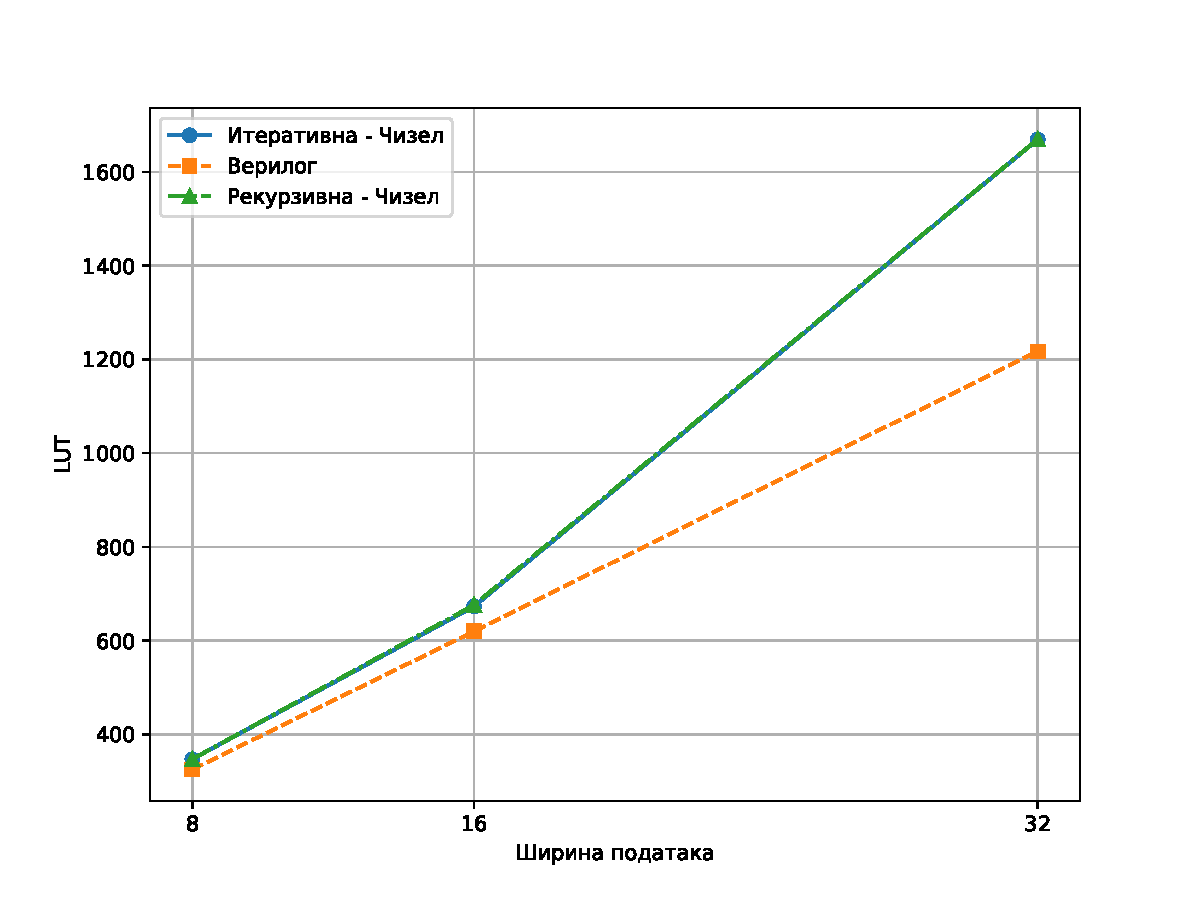
\includegraphics[scale=0.25]{slike/sorter_impl_LUTcomparison8.pdf}
      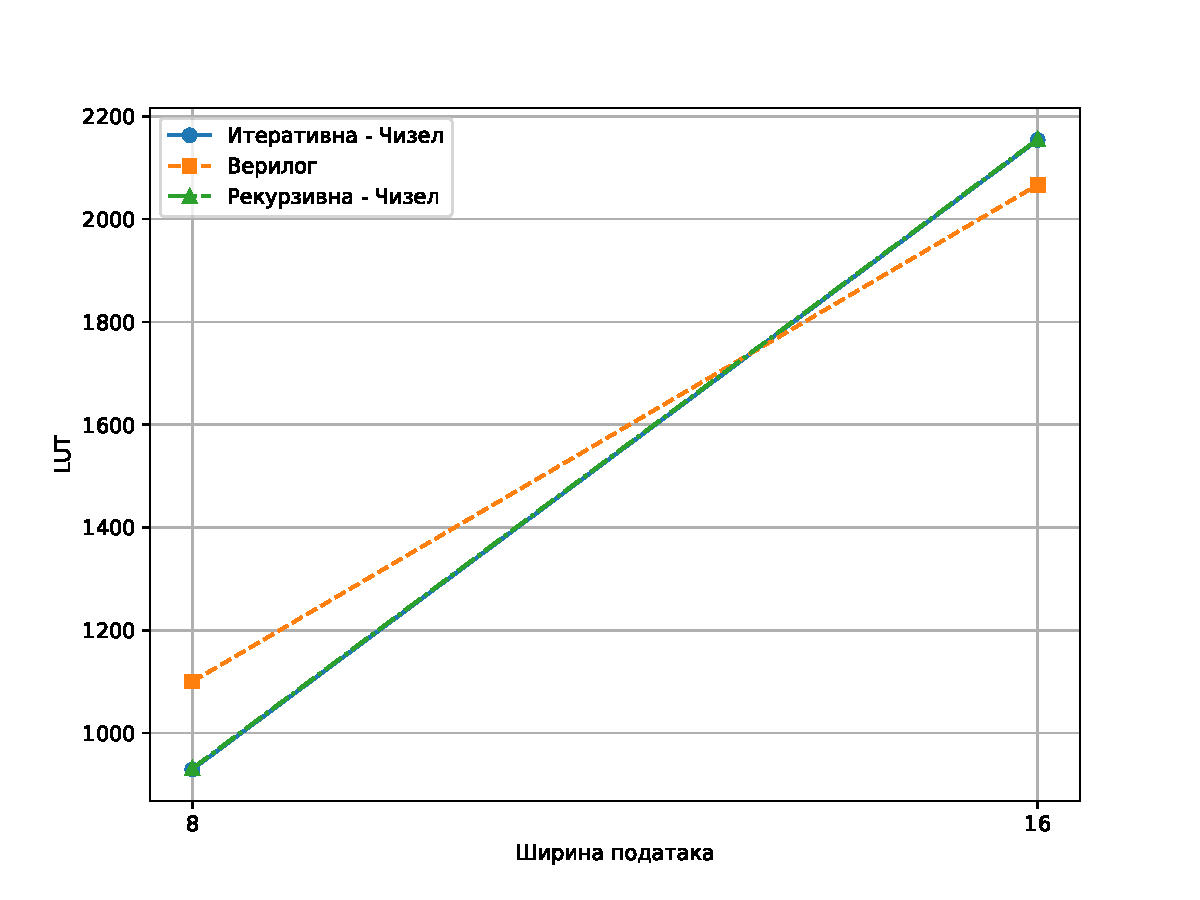
\includegraphics[scale=0.25]{slike/sorter_impl_LUTcomparison16.pdf}
 \end{figure}
\end{frame}

\begin{frame}%[fragile]
\frametitle{Поређење са претходним имплементацијама}
 \begin{itemize}
 \item Потрошња енергије изражена у [mW]
 \begin{table}[H]
\footnotesize
\centering
 \begin{tabular}{| c | c | c c c |}
  \hline
  Број ел. & Ширина & Вер. & Итер. & Рек. \\
  \hline
  8 & 8  & 530.08 & 530.06 & 531.20 \\
  8 & 16 & 535.70 & 535.81 & 536.66 \\
  8 & 32 & 546.12 & 546.50 & 545.98 \\
  \hline
  16 & 8 & 535.41 & 535.40 & 535.59 \\
  16 & 16 & 546.31 & 545.60 & 546.36 \\
  \hline
 \end{tabular}
 \label{tab:potrosnja}
\end{table}

 \item Број линија Верилог програмског кода
 \begin{table}[H]
  \footnotesize
  \centering
  \begin{tabular}{| c | c | c c |}
    \hline
    Број ел. & Ширина & Рекурзивна & Итеративна \\
    \hline
    8 & 8  & 356 & 327 \\
    8 & 16 & 368 & 327 \\
    8 & 32 & 368 & 327 \\
    \hline
    16 & 8 & 1158 & 1023 \\
    16 & 16 & 1158 & 1023 \\
    \hline
  \end{tabular}
  \end{table}

 \end{itemize}
\end{frame}

%%%%%%%%%%%%%%%%%%%%%%%%%%%%%%%%%%%%%%%%%%%%%%%%%%%%%%
%\section{Закључак}
\begin{frame}
\frametitle{Закључак}
\begin{itemize}
 \item Чизел нуди могућност дизајнирања хардвера са начином размишљања као да је у питању програмирање у језику вишег нивоа
 \item Рекурзивна имплементација битоник сортера заузима исти простор на чипу као итеративна
 \item Шема би била прегледнија ако би имплементација била састављена од подмодула, а не појединачних оператора
 \begin{itemize}
  \item Делује компликованије од итеративног решења, а сам програмски код је интуитивнији
 \end{itemize}
 \item Aнализирати битоник сорт алгоритам и уочити још неке начине рекурзивне имплементације чиме би се добила јаснија шема резултујућег кола
\end{itemize}
\end{frame}

\section{Хвала!}

% \begin{frame}[allowframebreaks]{Литература}
%
% \begin{thebibliography}{99}
%
% \bibitem{wiki_chisel}
% \textit{Chisel (programming language)}, приступљено (август 2023.) на
% \url{https://en.wikipedia.org/wiki/Chisel_(programming_language)}
%
% \bibitem{git_chisel}
% \textit{Chisel Bootcamp}, приступљено (август 2023.) на
% \url{https://github.com/freechipsproject/chisel-bootcamp.git}
%
% \bibitem{zuluaga2016}
%   Marcela Zuluaga, Peter Milder, and Markus Püschel,
%   ``Streaming sorting networks'',
%   ACM Trans.\ Des.\ Autom.\ Electron.\ Syst.\ 21, 4, чланак 55, 2016.
%   DOI: \url{http://dx.doi.org/10.1145/2854150}
%
% \bibitem{bitonicBatcher}
%   K.\ E.\ Batcher,
%   ``Sorting networks and their applications'',
%   ACM, 1968.
%   DOI: \url{http://dx.doi.org/10.1145/1468075.1468121}
%
% \bibitem{wiki_bitonic}
% \textit{Bitonic sorter}, приступљено (август 2023.) на
% \url{https://en.wikipedia.org/wiki/Bitonic_sorter}
%
% \bibitem{git_moj}
% \textit{BitonicSorterRecursive}, приступљено (септембар 2023.) на
% \url{https://github.com/aleksavelickovic5762015/BitonicSorterRecursive.git}
%
% \end{thebibliography}

%\end{frame}

\end{document}
